%%%%%%%%%%%%%%%%%%%%%%%%%%%%%%%%%%%%%%%%%%%%%%%%%%%%%%%%%%%%%%%%%%%%%%%
\setlength{\parindent}{0pt}
\setlength{\textheight}{22cm}
\setlength{\parskip}{0.2cm}

% Para aumentar o espa�amento entre as linhas
\linespread{1.2}
%%%%%%%%%%%%%%%%%%%%%%%%%%%%%%%%%%%%%%%%%%%%%%%%%%%%%%%%%%%%%%%%%%%%%%%

\chapter{Dom�nios de teste}

\section{PDDL - Linguagem de Defini��o de Do\-m�\-ni\-o de Planejamento}
\label{apendice_pddl}

Em 1998 foi criada a \ac{PDDL}\index{PDDL} \cite{McDermott1998}\cite{McDermott1998a}\cite{McDermott2000}. Esta linguagem tem como principal objetivo representar os dom�nios do mundo real por meio de uma estrutura capaz de ser entendida e interpretada por um planejador. A maioria dos planejadores desenvolvidos hoje s�o capazes de utilizar a \ac{PDDL} como representa��o de entrada do dom�nio para a gera��o de uma solu��o ou de um plano, j� que esta linguagem tornou-se um padr�o na �rea de planejamento autom�tico. A representa��o do modelo do dom�nio deve ser a mais pr�xima poss�vel do dom�nio real, contendo a descri��o das a��es poss�veis, suas pr� e p�s-condi��es, as informa��es sobre o estado inicial do dom�nio e o estado objetivo (metas), para que o planejador possa processar o modelo. \\

Algumas caracter�sticas principais da \ac{PDDL} s�o:


\chapter{Arquitetura do Sistema}
\label{apendice_arquitetura_sistema}

\section{Diagrama de implementa��o}

\begin{center}
  \begin{figure}[ht!]
    \centering
	\label{diagrama_classe}
    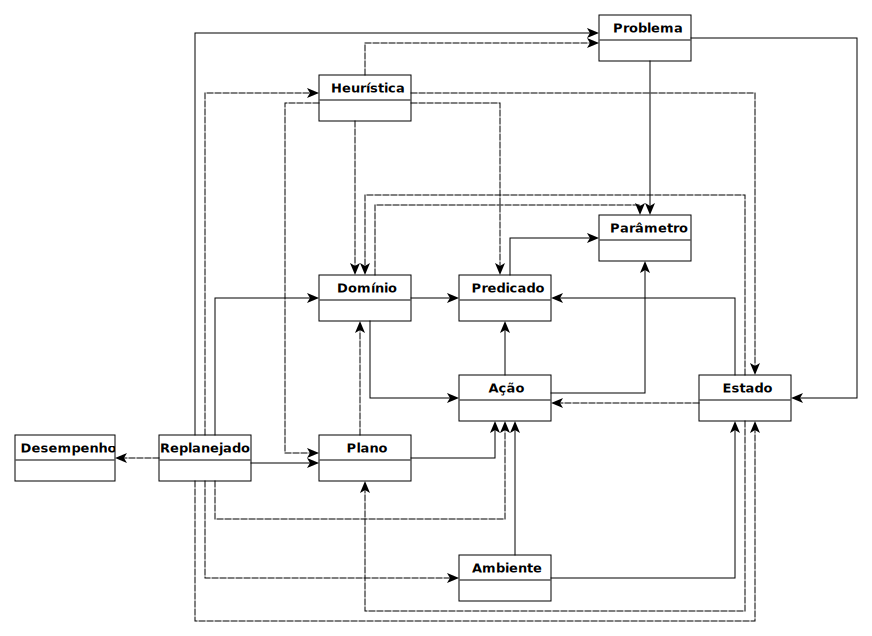
\includegraphics[angle=270,width=1.0\textwidth]{./img/diagrama_classe_sistema.ps}
    \caption[Diagrama de classe do sistema de reparo]{Diagrama de Classe\footnote{Este diagrama segue os conceitos apresentados por \cite{Martin2000}.} do sistema de reparo VHPOP-RE\index{VHPOP-RE}}
  \end{figure}
\end{center}
